\documentclass[11pt]{article}

% Change "review" to "final" to generate the final (sometimes called camera-ready) version.
% Change to "preprint" to generate a non-anonymous version with page numbers.
\usepackage[]{acl}
\usepackage{times}
\usepackage{latexsym}
\usepackage[T1]{fontenc}
\usepackage[utf8]{inputenc}
\usepackage{microtype}
\usepackage{inconsolata}
\usepackage{graphicx}
\usepackage{array}
\usepackage{xcolor}

\graphicspath{{figures/}}

% =====================================================================
% DRAFT NOTES
%   \todo{...}     red   - work still to do (rubric prompts live here)
%   \copynote{...} blue  - says what was carried over from the progress report
% Set \draftnotesfalse before submitting: every note disappears from the
% PDF. Then search this file for "\todo" to make sure none are left.
% =====================================================================
\newif\ifdraftnotes
\draftnotestrue
\ifdraftnotes
  \newcommand{\todo}[1]{{\color{red}\textbf{[TODO:} #1\textbf{]}}}
  \newcommand{\copynote}[1]{{\color{blue}\textit{[COPIED: #1]}}}
\else
  \newcommand{\todo}[1]{}
  \newcommand{\copynote}[1]{}
\fi

\title{Group 13 Final Report:\\Student Dropout Prediction}

\author{Jack Easton, Vikash Sasikumar, Michael Padeigis \\
  \texttt{\{eastoj2,sasikumv,padeigim\}@mcmaster.ca} }

\begin{document}
\maketitle

% \begin{abstract}
% \todo{Optional abstract, 4--6 sentences: task, data, best model, headline number, main error finding.}
% \end{abstract}

% =====================================================================
\section{Introduction}
% RUBRIC (10%, shared with Related Work): motivation + problem description,
% previous work, at least 7 references (at least 5 published studies),
% integrated into the discussion rather than listed. Also answer: did related
% work change our direction after the progress report?
% ---------------------------------------------------------------------
% COPIED FROM PROGRESS REPORT: Section 1 "Introduction", unchanged.
% =====================================================================
\copynote{Progress Report \S1 Introduction, unchanged.}

With the rising prevalence of AI use in education, there has been a cause for concern with regards to the negative impacts it has on students. Studies have shown that by cognitively offloading their thinking and outsourcing their work, students have eroded their mental abilities and have caused significant reduction in brain activity \citep{hogenboom2026}. However, this is not the only way machine learning has to be used in education. By using student information available at enrollment and after the first semester to predict dropout versus graduation, machine learning can help identify students who may benefit from academic support.

\todo{Expand the problem statement: state the task precisely (binary Dropout vs Graduate at two time points, plus the 3-class variant if it is run), why early prediction matters (time to intervene), and a one-paragraph preview of what this report contributes and finds.}

\todo{References check. \texttt{hogenboom2026} is an online article, not a published study. We currently cite 6 published studies (vaarma2024, martinez2024, goren2024, niemi2012, rabelo2025, realinho2022data) and 8 sources in total, which meets the minimum. Consider adding 1--2 more, ideally prior work that reports results on this exact UCI dataset, so it can serve as a comparison point in Implementation.}

% =====================================================================
\section{Related Work}
% COPIED FROM PROGRESS REPORT: Section 2 "Related Work", all five
% paragraphs unchanged.
% =====================================================================
\copynote{Progress Report \S2 Related Work, all five paragraphs unchanged.}

The research paper ``Predicting student dropouts with machine learning: An empirical study in Finnish higher education'' by Matti Vaarma found the features ``accumulated credits'', the ``number of failed courses'', and ``Moodle activity count'' to be the most important features \citep{vaarma2024}. They found that up until 20 months, ``number of failed courses'' was the most important feature then afterward ``accumulated credits'' became the most important feature \citep{vaarma2024}. Then the study found that after 41 months, the reliability of all the features fluctuates \citep{vaarma2024}. These fluctuations happen in time intervals shorter than a semester \citep{vaarma2024}. They found that GPA and gender had little importance \citep{vaarma2024}.

The research paper ``Prediction of student dropout using Artificial Intelligence algorithms'' by Jairo Martínez and Dodanim Castillo found that socioeconomic data along with academic data accurately predicts student dropout rates \citep{martínez2024}. However, the study did not use any economic data about the students or their parents \citep{martínez2024}. Their model found that using data from just the first was sufficient and that using data from more years only found slight improvements in accuracy \citep{martínez2024}.

The research paper ``Early Prediction of Student Dropout in Higher Education using Machine Learning Models'' by Or Goren, Liron Cohen, and Amir Rubinstein used Learning Management System (LMS) data \citep{goren2024}. LMS tracks student learning activities which includes grades, submission times, forum participation, and more \citep{goren2024}. The researchers divided up their data by looking at the first 4 weeks, then the first 8 weeks, then the first exam period in semester 1, then the second exam period in semester 1 when the final semester 1 grade is available, and then finally they looked at the end of semester 2 data \citep{goren2024}. They found that with more data, the model became more accurate \citep{goren2024}. However, that also means there is less time to intervene when it seems a student may drop out \citep{goren2024}. The researchers also found that the dropout patterns changed depending on the field of study of the students \citep{goren2024}.

The research paper ``Using Big Data to Predict Student Dropouts: Technology Affordances for Research'' by David Niemi and Elena Gitin found that declining performance was a good indicator of dropping out and having dependents, being married or in the military reduced the likelihood of dropping out \citep{niemi2012}. They found that being older, and having previous college education or having transfer credits increased risk of dropping out \citep{niemi2012}.

The research paper ``A model for predicting dropout of higher education students'' by Anaíle Mendes Rabelo and Luis Enrique Zárate found that a high percentage of cancelled courses, fewer semesters enrolled, a low percentage of courses completed, loss of discounts and scholarships, and low GPA were among the features that correlated with higher dropout rates \citep{rabelo2025}. Unlike the previous studies, these researchers also tried to predict when a student might drop out. However, they found that these features were not useful for predicting that \citep{rabelo2025}.

\todo{Tie each paper back to OUR choices instead of only summarising it. For example: Goren et al.\ motivate our two prediction times (enrollment vs.\ after semester 1); Vaarma's failed-courses finding motivates the zero-approved-units indicator; Goren's field-of-study finding motivates breaking errors down by Course in Error Analysis.}

\todo{Add a short paragraph answering: did anything we read after the progress report change our direction? If nothing did, say why the original plan still held.}

% =====================================================================
\section{Dataset}\label{sec:dataset}
% RUBRIC (5%): dataset properties and preprocessing. If the dataset changed
% since the progress report, describe the change in its own subsection.
% ---------------------------------------------------------------------
% COPIED FROM PROGRESS REPORT: Section 3 "Dataset" (Source, Properties,
% Table 1, Notable Characteristics, Preprocessing), unchanged.
% NEW: subsection "Changes Since the Progress Report".
% =====================================================================
\copynote{Progress Report \S3 Dataset, all subsections and Table~\ref{tab:feature-groups} unchanged.}

\subsection{Source}

We use the ``Predict Students' Dropout and Academic Success'' dataset from the UCI Machine Learning Repository \citep{realinho2021uci}, which was donated by the Instituto Polit\'{e}cnico de Portalegre in Portugal \citep{realinho2022data}.
It covers undergraduates in 17 degree programs.
The records were compiled from the institution's academic and admissions databases and combined with national macroeconomic indicators.
The donors had already cleaned the data and integer-encoded the categorical fields, so we did not need to annotate anything.

\subsection{Properties}

The dataset has 4,424 instances, one per student.
Each has 36 input features and one target label.
There are no missing values and no duplicate rows.
Table~\ref{tab:feature-groups} groups the features.
Eight are binary and nine are nominal categorical, stored as integer codes with no inherent order.
The rest are numeric or counts.
Semester grades use the Portuguese 0--20 scale.
Admission and previous-qualification grades use a 0--200 scale (observed range 95--190).

\begin{table}[t]
  \centering
  \small
  \setlength{\tabcolsep}{4pt}
  \begin{tabular}{l>{\raggedright\arraybackslash}p{4.3cm}r}
    \hline
    \textbf{Group} & \textbf{Examples} & \textbf{\#} \\
    \hline
    Demographic   & gender, age at enrollment, nationality, displaced & 7 \\
    Socioeconomic & parents' qualification/occupation, debtor, scholarship & 7 \\
    Enrollment    & course, application mode/order, admission grade & 7 \\
    Academic      & per semester: units credited, enrolled, evaluated and approved; grade; units without evaluations & 12 \\
    Macroeconomic & unemployment rate, inflation rate, GDP & 3 \\
    \hline
  \end{tabular}
  \caption{\label{tab:feature-groups}
    The 36 input features, grouped by type.
  }
\end{table}

The target is one of three outcomes: Graduate (2,209; 49.9\%), Dropout (1,421; 32.1\%) or Enrolled (794; 17.9\%).
The majority-class baseline reaches about 50\% accuracy on the original three class dataset and 60.9\% on our binary test set after excluding Enrolled students.
We therefore report dropout recall, precision and F1 alongside accuracy, as described in Section~\ref{sec:evaluation}.

\subsection{Notable Characteristics}

Following our TA's suggestion to look closely at anomalies, we examined each feature's distribution and found several properties that affect modelling.

\begin{itemize}
  \item \textbf{Zero grades:} 718 students have a first-semester grade of 0, and 870 have a second-semester grade of 0.
    All students with a zero semester grade also had zero approved units, although some had recorded evaluations.
    Among students with a zero first semester grade, approximately 79\% are classified as Dropout, so the feature is highly predictive, but its zero value means something different from the rest of the grade scale.
  \item \textbf{Skewed categoricals:} 97.5\% of students share the same nationality, and 89\% are single.
    Only 51 students have educational special needs.
    Several coded features also have many values (father's occupation has 46 codes, mother's qualification has 29), and many of those codes are rare.
  \item \textbf{Age:} age is right-skewed.
    The median is 20 and the range is 17--70, with 662 students older than 30.
  \item \textbf{Macroeconomic features:} each has only about 10 distinct values because they are tied to the year of enrollment.
    They act more like a cohort indicator than a continuous measurement.
\end{itemize}

\subsection{Preprocessing}

The raw CSV needed some cleanup before use.
We removed 73 empty trailing columns left over from the export, stripped a UTF-8 byte-order mark from the first header, and removed a stray tab character from the ``Daytime/evening attendance'' column name.
We excluded the 794 Enrolled students because their final outcomes were unknown. This left 3,630 students, with Dropout\,=\,1 and Graduate\,=\,0.

We kept the zero-grade students and the older students.
Both are real records rather than errors, and the zero-grade group carries a strong dropout signal.
No additional rows were removed.
We split the data 80/20 into training and test sets, stratified by class.
Any scaling or encoding was fit on the training set only, to avoid leaking test data.
Section~\ref{sec:features} describes how the categorical and numeric features are represented, and Section~\ref{sec:evaluation} describes the evaluation protocol.

The data file (\texttt{data.csv}, about 0.8\,MB) is included in our submission.

\subsection{Changes Since the Progress Report}

\todo{Describe any data changes since the progress report. Likely candidates: (1) the three-class experiment (exp5) keeps the 794 Enrolled students, so give its class counts and split here; (2) the derived zero-approved-units indicator (exp4). If the binary dataset itself is unchanged, say so in one sentence.}

% =====================================================================
\section{Features and Inputs}\label{sec:features}
% RUBRIC (5%): model inputs, feature engineering and why, feature
% selection/augmentation, and how features were VARIED across experiments.
% ---------------------------------------------------------------------
% COPIED FROM PROGRESS REPORT: Section 4 "Features" (3 paragraphs), unchanged.
% NEW: engineered features and the ablation design.
% =====================================================================
\copynote{Progress Report \S4 Features, unchanged.}

We used two feature sets to compare dropout prediction at enrollment and after the first semester. The enrollment model used 24 features, including demographic information, admission details, previous qualifications, financial indicators and economic conditions. It excluded academic results from both semesters.

The first semester model added six academic measures, giving 30 features. These included curricular units credited, enrolled, evaluated and approved, the semester grade, and units without evaluations. Results from the second semester were excluded from both models.

Categorical features were represented using one hot encoding, while numerical features were standardized. These transformations were fitted within the training folds during cross validation. Feature selection was based on the intended prediction stage. We did not use automatic feature selection or data augmentation.

\subsection{Engineered Features}

\todo{Describe the zero-approved-units indicator (exp4): definition, motivation (a grade of 0 means "no units approved", not "very low grade"; see Notable Characteristics), and any other engineered features (e.g.\ approved/enrolled ratio, grade missing-indicator). Explain WHY each one should help.}

\subsection{Feature Ablations}

\todo{Describe how the inputs were varied: removing one feature group at a time from Table~\ref{tab:feature-groups} (and/or adding one at a time), with and without the engineered features. Point to the ablation results table in Section~\ref{sec:implementation} or Section~\ref{sec:error}. Output: \texttt{outputs/experiments/exp4\_features\_ablation/}.}

% =====================================================================
\section{Implementation}\label{sec:implementation}
% RUBRIC (20%): several models/versions; simple baseline (majority) plus at
% least one trained baseline that we beat (or explain why not); loss
% function; optimisation technique; ablations for complex models.
% ---------------------------------------------------------------------
% COPIED FROM PROGRESS REPORT: Section 5 "Implementation" (4 paragraphs),
% unchanged. NEW: hyperparameter tuning, controlled comparison, threshold
% tuning, three-class model.
% =====================================================================
\copynote{Progress Report \S5 Implementation, unchanged.}

We built a binary classifier to predict whether a student would drop out or graduate. We excluded students who were still enrolled because their final outcomes were not known. We tested two versions using the same train and test split. The enrollment version used 24 features available before semester results. The first-semester version used 30 features by adding six first-semester academic measures.

We compared four scikit-learn models: logistic regression, a decision tree, a random forest, and a support vector machine (SVM). All four used balanced class weights, giving more weight to dropout cases because they were less common. Each model used a preprocessing pipeline that encoded categorical features and standardized numerical features. We fitted these transformations on the training portion of each fold to keep the validation data separate.

Logistic regression minimized logistic loss with L2 regularization using the L-BFGS optimizer. The decision tree chose splits that reduced Gini impurity, with a maximum depth of seven and at least 15 examples per leaf. The random forest averaged predictions from 200 trees trained on bootstrap samples, with each split considering a random subset. The SVM used a radial basis function kernel with C = 1. It learned a decision boundary by balancing the width of the classification margin against penalties for margin violations. We enabled probability estimates so the SVM could produce dropout risk scores.

For comparison, we used a majority class baseline. The training set contained 1,767 graduates and 1,137 dropouts, so the baseline predicted Graduate for every student in the test set.

\subsection{Hyperparameter Tuning}

\todo{exp2: describe the search (grid or random), the ranges for each model (e.g.\ LR $C$; tree depth and min leaf; RF number of trees, depth, max features; SVM $C$ and $\gamma$), the selection metric (ROC-AUC on the 5 training folds), and the chosen values. Give a small table: hand-set vs.\ tuned CV score.}

\subsection{Controlled Comparison Across Feature Sets}

\todo{exp1: train ALL FOUR algorithms on BOTH feature sets with identical settings, so the gain from first-semester data is not mixed up with the change of model (LR $\rightarrow$ SVM). Report a $4 \times 2$ table of test ROC-AUC / recall / F1.}

\subsection{Decision Threshold}

\todo{exp3: the progress report used a fixed 0.50 cutoff. Explain how the cutoff was chosen from out-of-fold training predictions (e.g.\ maximise F1, or fix dropout recall $\geq 0.90$), and why missing an at-risk student costs more than a false alarm.}

\subsection{Three-Class Model}

\todo{exp5: the same pipeline on Dropout / Enrolled / Graduate. Loss (multinomial log-loss for LR), class weights, and what changes in the setup. Results go in Section~\ref{sec:evaluation}.}

\todo{State plainly which model is "ours" (final) versus the baselines: majority baseline, plus at least one trained baseline (e.g.\ untuned logistic regression or decision tree). Confirm ours beats both; if it does not, explain why (this can be expanded in Error Analysis).}

% =====================================================================
\section{Evaluation}\label{sec:evaluation}
% RUBRIC (15%): evaluation strategy; train/val/test split SIZES and LABEL
% DISTRIBUTIONS; cross-validation; metrics; were the progress-report
% metrics adequate?
% ---------------------------------------------------------------------
% COPIED FROM PROGRESS REPORT: Section 6 "Results and Evaluation", the
% split and protocol paragraphs, plus the existing numbers (moved into
% Table 2). NEW: split table, metrics-adequacy discussion, new results.
% =====================================================================
\copynote{Progress Report \S6 Results and Evaluation, protocol paragraphs and existing test numbers (now in Table~\ref{tab:results}).}

We split the 3,630 students with known outcomes into 2,904 training examples (80\%) and 726 test examples (20\%). We compared the four models using stratified five fold cross-validation within the training set. For each feature set, we selected the model with the highest mean validation ROC-AUC, trained it on all 2,904 training examples, and evaluated it on the test set. Logistic regression had the highest mean validation ROC-AUC at enrollment (0.848), and the SVM had the highest after the first semester (0.934).

We treated dropout as the positive class. We used ROC-AUC to measure how well each model ranked dropout cases above graduates across decision thresholds. We used a dropout probability cutoff of 0.50 to calculate accuracy, precision, recall, and F1.

\begin{table}[t]
  \centering
  \small
  \setlength{\tabcolsep}{3pt}
  \begin{tabular}{lrrrr}
    \hline
    \textbf{Split} & \textbf{Total} & \textbf{Dropout} & \textbf{Graduate} & \textbf{Enrolled} \\
    \hline
    Train (binary) & 2,904 & 1,137 & 1,767 & -- \\
    Test (binary)  & 726   & 284   & 442   & -- \\
    Train (3-class) & \todo{} & \todo{} & \todo{} & \todo{} \\
    Test (3-class)  & \todo{} & \todo{} & \todo{} & \todo{} \\
    \hline
  \end{tabular}
  \caption{\label{tab:splits}
    Split sizes and label distributions. Validation uses 5 stratified folds inside the training set (about 581 per fold).
  }
\end{table}

\begin{table*}[t]
  \centering
  \small
  \begin{tabular}{llrrrrr}
    \hline
    \textbf{Prediction time} & \textbf{Model} & \textbf{ROC-AUC} & \textbf{Recall} & \textbf{Precision} & \textbf{F1} & \textbf{Accuracy} \\
    \hline
    any & Majority baseline & 0.500 & 0.000 & -- & 0.000 & 0.609 \\
    Enrollment & Logistic regression (progress report) & 0.855 & 0.775 & 0.673 & 0.720 & 0.764 \\
    After sem.\ 1 & SVM (progress report) & 0.956 & 0.887 & 0.890 & 0.889 & 0.913 \\
    \hline
    Enrollment & \todo{tuned model} & & & & & \\
    After sem.\ 1 & \todo{tuned model} & & & & & \\
    After sem.\ 1 & \todo{tuned model + tuned cutoff} & & & & & \\
    \hline
  \end{tabular}
  \caption{\label{tab:results}
    Held-out test results (726 students, dropout = positive class, cutoff 0.50 unless stated). Top block copied from the progress report; bottom block to be filled in from the experiments.
  }
\end{table*}

The baseline classified all 442 graduates correctly and missed all 284 dropout cases, showing why we looked at recall alongside accuracy. The enrollment model identified 220 dropout cases, while the first-semester model identified 252.

\todo{Three-class results: macro-F1 and per-class recall (exp5), compared with the binary setup, and with prior published results on this dataset if available.}

\todo{Metrics adequacy: were the progress-report metrics enough? Discuss: accuracy is misleading at 61\% majority; ROC-AUC ignores the operating point; PR-AUC / average precision suits the minority class; macro-F1 for 3-class; possibly calibration (Brier score is already saved in \texttt{metrics.json}).}

% =====================================================================
\section{Progress}\label{sec:progress}
% RUBRIC (10%): reflect on the progress-report plan. Did we follow
% through? Did the plan change? Why?
% ---------------------------------------------------------------------
% NEW SECTION. The five items below are the plan from Progress Report
% Section 7 "Feedback and Plans" (that section is removed in the final).
% =====================================================================

In the progress report we committed to five follow-up items. We discuss each in turn.

\todo{For each item: was it done? What did we find? Did the plan change, and why? One short paragraph each.}

\begin{itemize}
  \item \textbf{Enrolled class (three-class setup):} \todo{status and outcome, exp5.}
  \item \textbf{Decision cutoff tuning and precision--recall curves:} \todo{status and outcome, exp3.}
  \item \textbf{Hyperparameter tuning with cross-validation:} \todo{status and outcome, exp2.}
  \item \textbf{Zero-grade indicator:} \todo{status and outcome, exp4.}
  \item \textbf{Controlled comparison (same algorithm, both feature sets):} \todo{status and outcome, exp1.}
\end{itemize}

\todo{Mention anything done that was NOT in the plan (e.g.\ feature-group ablations, error analysis by subgroup) and anything planned but dropped, with the reason.}

% =====================================================================
\section{Error Analysis}\label{sec:error}
% RUBRIC (20%, the largest single section): systematic error examination
% with figures/stats/examples (confusion matrices, high-error test cases).
% What is the model good/bad at? How do models differ? Error patterns?
% What would we do next to fix them?
% ---------------------------------------------------------------------
% NEW SECTION. Figures copied from Student_Risk_ML/outputs/*/confusion_matrix.png
% Supporting analysis: exp6_error_analysis.py
% =====================================================================

\todo{Opening paragraph: describe the method. Which model(s) are analysed, on which split, and the steps (confusion matrices, then the highest-error cases, then error rates by subgroup, then a comparison between models).}

\begin{figure}[t]
  \centering
  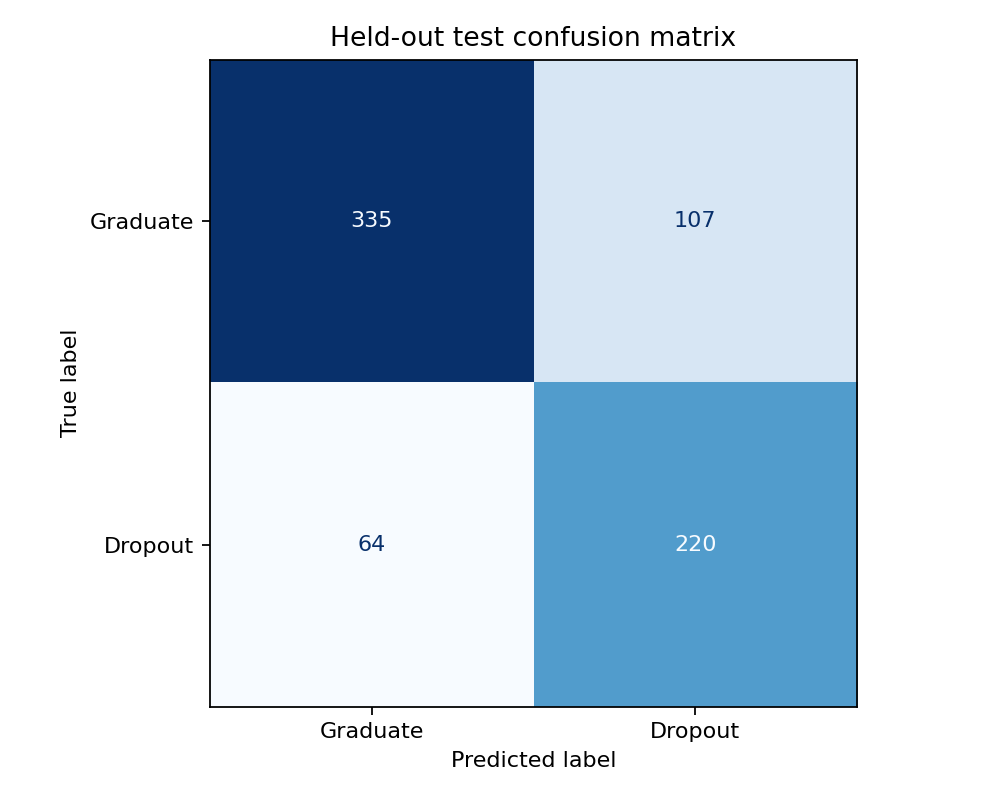
\includegraphics[width=0.49\columnwidth]{cm_enrollment.png}
  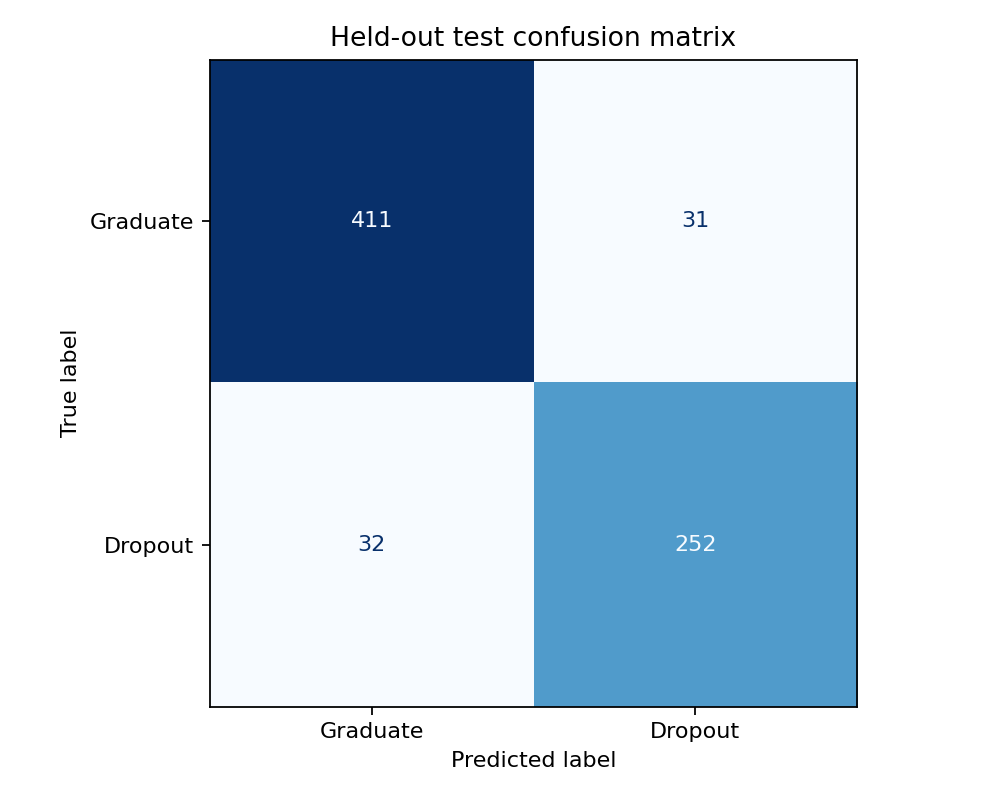
\includegraphics[width=0.49\columnwidth]{cm_after_first_semester.png}
  \caption{\label{fig:cm}
    Test-set confusion matrices at enrollment (left, logistic regression) and after the first semester (right, SVM), cutoff 0.50. \todo{Replace these with the final models' matrices if the models change.}
  }
\end{figure}

\subsection{Overall Error Profile}

\todo{Read Figure~\ref{fig:cm}: false negatives (missed dropouts) vs.\ false positives at each prediction time. Which kind of error dominates, and which matters more for the use case?}

\subsection{High-Error Test Cases}

\todo{Table of 5--8 test students with the most confident wrong predictions (e.g.\ graduate given $p \geq 0.9$, or dropout given $p \leq 0.1$). Show a few key features for each. What do they have in common? (exp6 writes \texttt{high\_error\_cases.csv}.)}

\subsection{Errors by Subgroup}

\todo{Error rate / recall by Course, age band, zero-grade vs.\ non-zero, scholarship, debtor, tuition up to date (exp6 writes \texttt{errors\_by\_subgroup.csv}). Where is the model good, and where is it bad? Connect to Goren et al.'s field-of-study finding.}

\subsection{Model Comparison}

\todo{How do the errors of the enrollment and first-semester models differ? Which students are caught only once semester-1 data arrives? Which are still missed? If the 3-class model is run: where does Enrolled get confused?}

\subsection{Future Fixes}

\todo{For each error pattern above, one concrete fix we would try next (e.g.\ per-course models or interaction features, calibrated thresholds per subgroup, a mid-semester time point, more data for small courses).}

% \section*{Limitations}
% \todo{Optional: single institution, cohort effects, fairness of demographic features, observational target.}

% =====================================================================
\section*{Team Contributions}
% RUBRIC (5%): at least one sentence per member; do NOT write "all members
% contributed equally".
% ---------------------------------------------------------------------
% PROGRESS REPORT VERSION (for reference only; rewrite for the final):
%   Vikash: Introduction, cited 5 previous works, Features section, ML pipeline.
%   Michael: developed ML pipeline, trained and evaluated models, wrote
%            Implementation and Results and Evaluation.
%   Jack: LaTeX setup, explored/preprocessed dataset, wrote Dataset and
%         Feedback and Plans, helped with ML pipeline, reviewed report.
% =====================================================================

\todo{At least one sentence per member covering the WHOLE project (progress-report work plus final-report work). Do not write "all members contributed equally".}

Jack: \todo{}

Vikash: \todo{}

Michael: \todo{}

\bibliography{custom}

\end{document}
